\chapter{The Ahuora Digital Twin Platform}


%This chapter has been included based on feedback from the mid-progress report that the marker did not understand the context of the project.
\textit{ The work presented in this report is part of a larger, multi-disciplinary project. Consequently, some of the presented work goes beyond the limited scope of this immediate research, but is still required to achieve outcomes relating to the integration of live data analysis into the broader software platform. As such, this content is still relevant within the context of this specific project. Additionally, some work involves research for future implementations that cannot be completed with the platform's current capabilities. This chapter provides an overview of the Ahuora Digital Twin Platform, to provide context for the rest of the report.}

\section{Background}

`Project Ahuora' is a Ministry of Business, Innovation and Employment (MBIE) funded project that aims to decarbonise the process heat sector.
By decarbonising, New Zealands' greenhouse gas emissions will be reduced. Cost savings from reduced energy consumption are anticipated, along with increased energy independence.
This is a multi-disciplinary project that involves researchers from the University of Waikato, University of Auckland, Massey University,
and other global universities. Chemical Engineers bring understanding of the chemical processes that are used in industry. Electrical Engineers bring understanding of the grid system
and how to integrate renewable energy sources. Mechanical engineers bring understanding of how to design and build more efficient systems. Software Engineers bring understanding of how to
model, simulate, and monitor complex systems.

A key objective is to develop a digital twin platform for the chemical processing industry. This platform will allow New Zealand factory operators to model their processes, simulate different scenarios, and monitor process state in real-time.
This will enable factory operators to make data-driven and scientifically backed decisions on how to improve their processes. A digital twin can recognise where the factory is underperforming, suggest real-time improvements, and help plain future investments.

\section{The Ahuora Simulation Platform}

A key deliverable of the Ahuora project to date is the Ahuora Simulation Platform. This is a web-based platform that allows users to model a factory or other energy system, and simulate its performance. Much of the analysis functionality is achieved by leveragin the IDAES Process Systems Engineering framework within the backend. IDAES is a Python library that provides tools for modelling and simulating chemical processes.

Currently, the platform can model a factory at a single point in time. The user specifies the properties of the factory, such as the flow rates of different materials, the temperature and pressure of different streams, and the efficiency of different unit operations. The platform then simulates the factory and provides the user with a report on the factory's performance.

\subsection{Flowsheet Interface}


\begin{figure}
    \centering
    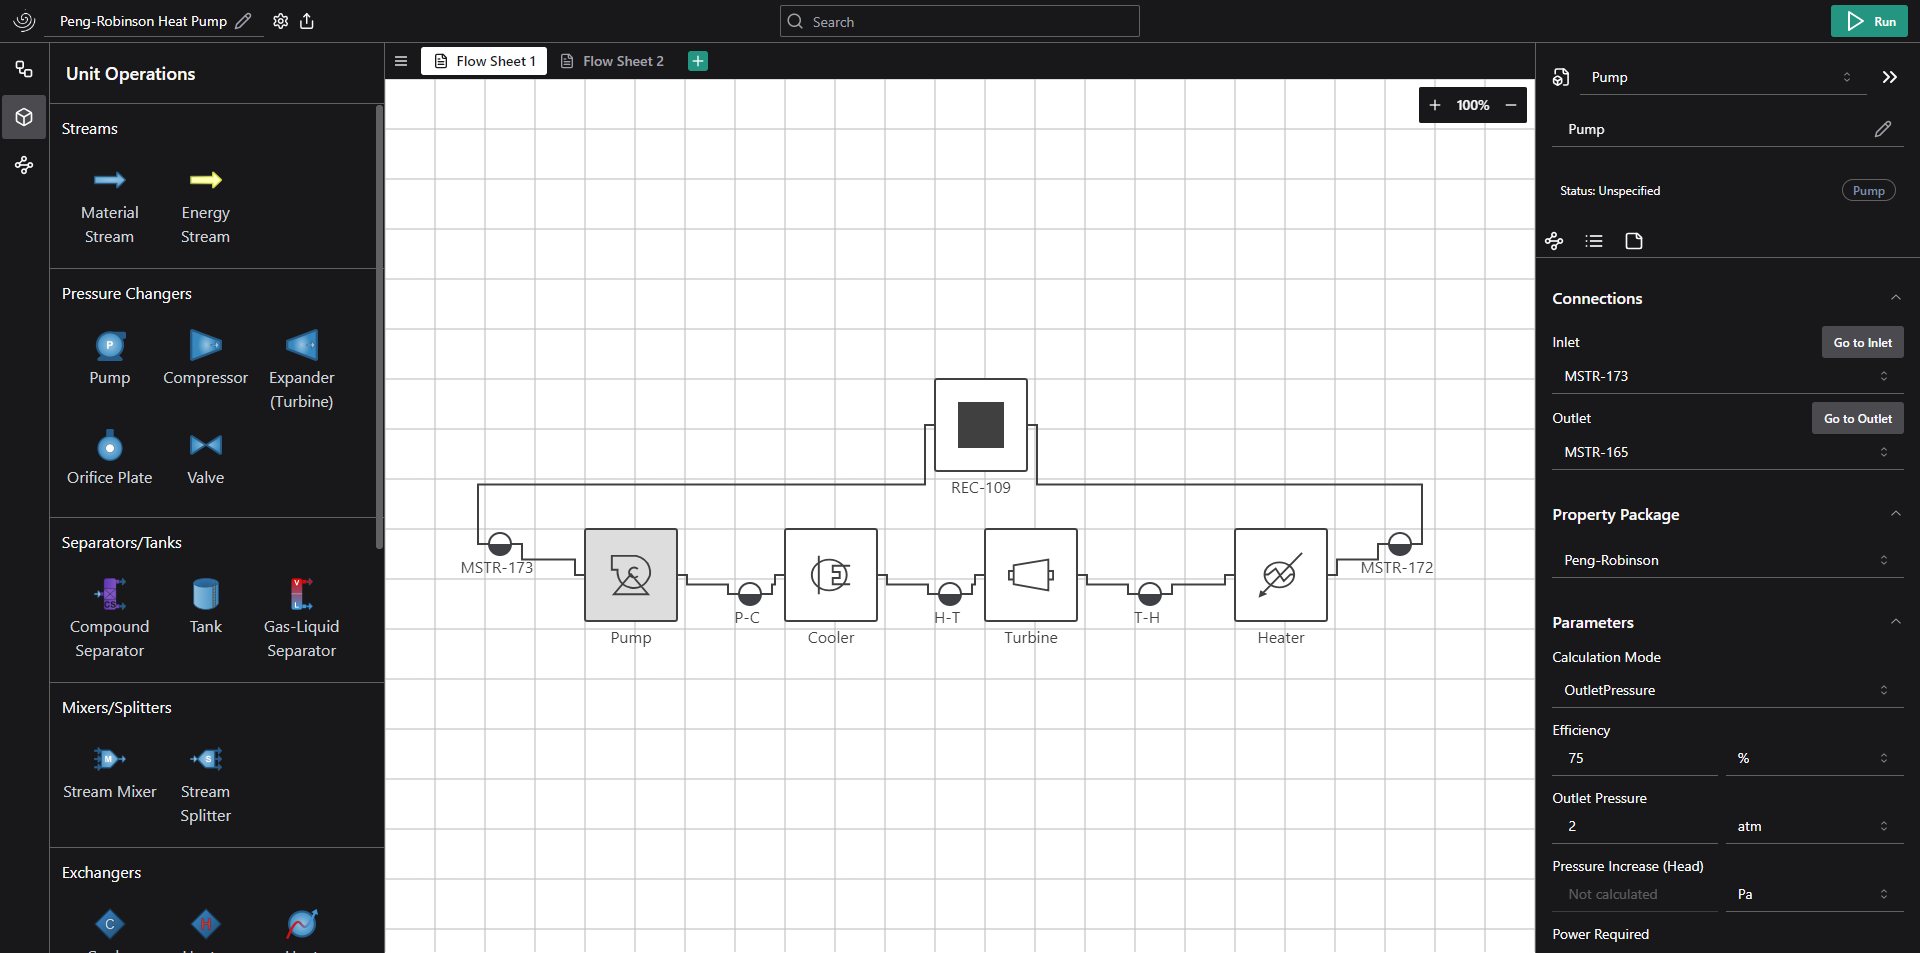
\includegraphics[width=\textwidth]{platform_screenshot.png}
    \caption{Example Flowsheet in the Ahuora Simulation Platform}
    \label{fig:platform}
\end{figure}

\Cref{fig:platform} shows a screenshot of the Ahuora Simulation Platform, as at August 2024. The user interface is divided into three main sections. The left-hand panel shows a list of unit operations from a factory, including pumps, heaters, heat exchangers, reactors, and material streams. The user can drag and drop these unit operations onto the canvas in the centre of the screen. The user can then connect the unit operations together to create a process flow diagram. The right-hand panel shows the properties of the selected unit operation, such as the flow rate of the material stream, the temperature and pressure of the stream, and the efficiency of the unit operation. The user can edit these properties to simulate different scenarios.

The displayed flowsheet shows a simple heat pump cycle. The block on the top is a ``recycle", specifying that the output of the cooler is fed back into the pump. A more complex flowsheet would replace the cooler and heater with heat exchangers, which exchange heat with their environment, but this provides a simple example.

\subsection{Online Integration}

\begin{figure}
    \centering
    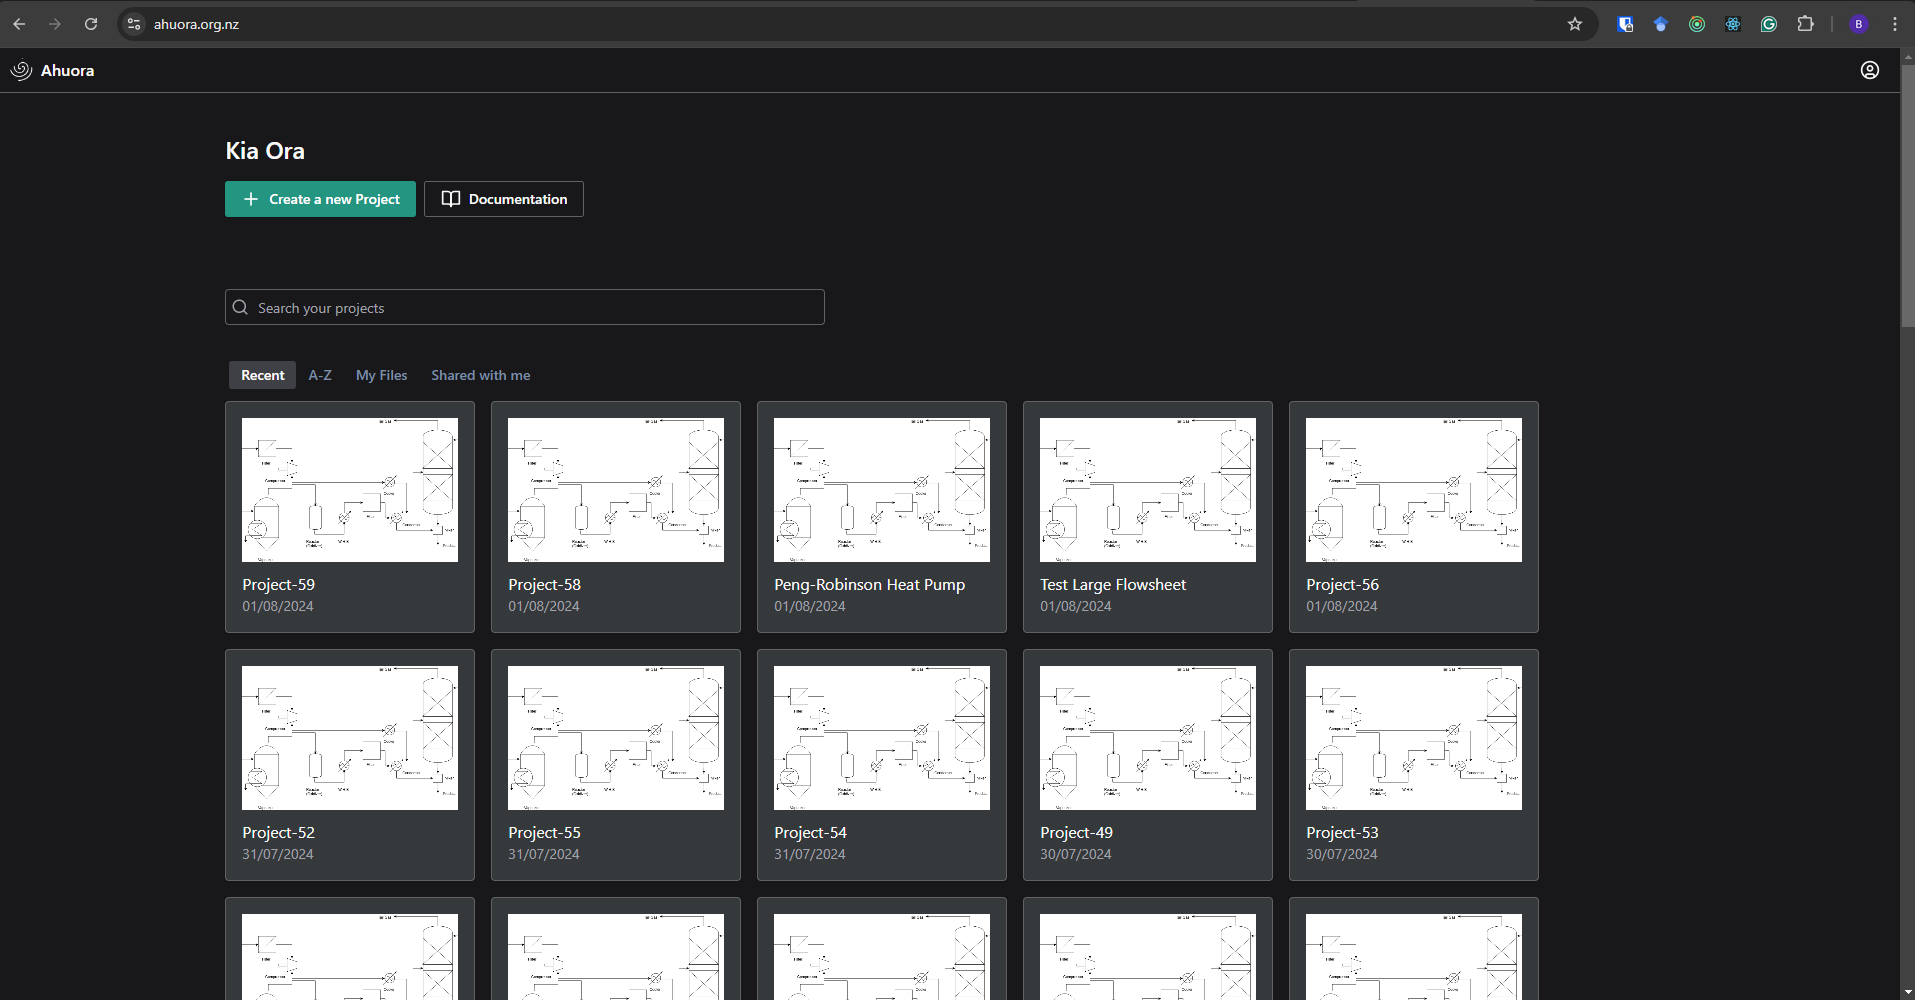
\includegraphics[width=\textwidth]{platform_homepage.png}
    \caption{Homepage of The Ahuora Simulation Platform}
    \label{fig:homepage}
\end{figure}

The Ahuora Simulation Platform is designed as a web-based multi-user platform. This offloads processing and data storage to the server, allowing users to access the platform from any device with a web browser. Simulation can be very computationally expensive, particuarly in advanced models, so this is a key feature. It enables simulation to be run in parallel on powerful servers, as the simulation is not done within the local web browser, but rather via distributed server infrastructure. This allows the platform to be used in industry without requiring significant upfront investment in hardware. 

In future, this will also enable the platform to be used for real-time collaboration between multiple users. Its API allows it to be integrated with other software, enabling enhanced functionality, real-time updates, and broader interactions.

The home page of the platform, shown in \Cref{fig:homepage}, provides a list of saved simulations, and allows the user to create a new simulation. This is not publicly acessible, as the platform is still in development, and user account functionality is not yet complete.

\section{Platform Architecture}

\begin{figure}[h]
    \centering
    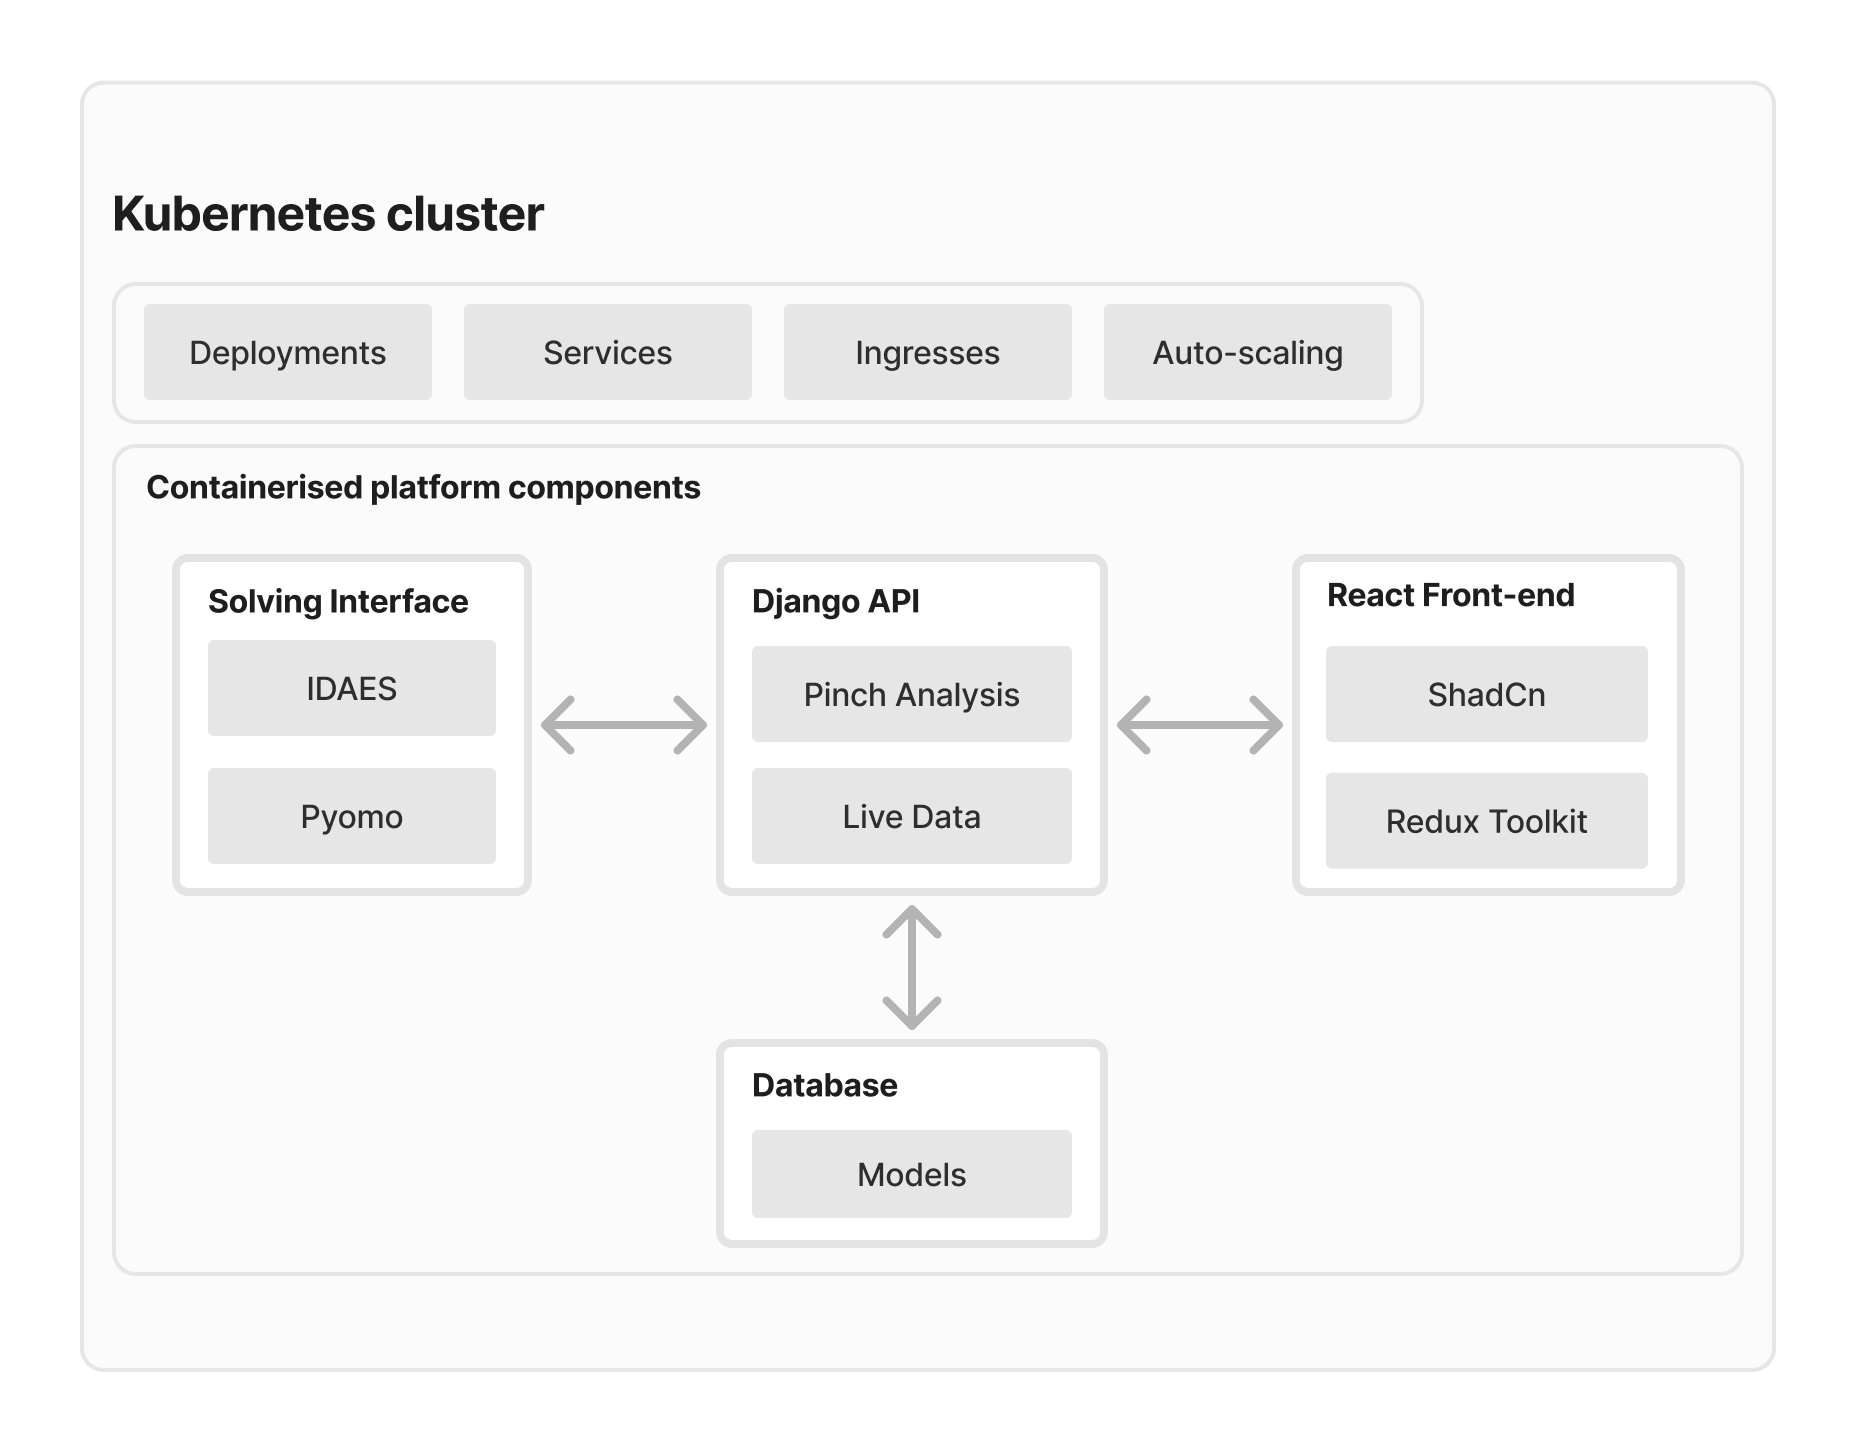
\includegraphics[width=\textwidth]{dt_arch.png}
    \caption{Architecture of the Ahuora Digital Twin Platform}
    \label{sec:platform_architecture}
\end{figure}

The platform is hosted in a Kubernetes cluster, located on-site. The Kubernetes cluster handles all web traffic, deployments from the private Github Repository, and scaling of services. 

Within the platform there are various containers running through the Docker platform, that can be replicated as required to scale based on service demand. The Database stores all flowsheets and model data. The solving interface uses the IDAES Process Simulation software~\cite{lee2021idaes}, built on the Pyomo equation-oriented modelling language~\cite{bynum2021pyomo}, to simulate a factory in real time. The User Interface is written in React Typescript, and uses the ShadCN UI Library and Redux Toolkit for state management and communication with the Django Backend. The Django API links all the services together, and handles the business logic for functionality such as Pinch Analysis and Live Data processing.

\section{Ongoing Projects}

Multiple other projects are being completed in parallel by other team members. Each project has a distinct topic, and is largely independent, but collaboration is required to ensure that each other's work is compatible.The projects cover a variety of topics, from analyis and data processing, to usability and deployment.

\subsection{Live Data Processing}

\textbf{Team Member Responsible:} Bert Downs

The Ahuora Platform currently supports building and simulating a factory, but it has no functionality to link live data from a factory into the Ahuora Platform. By integrating real-time sensor data into the simulation, the platform can monitor the factories' performance, and suggest tunings that will optimise resource efficiency. The data can also be used to predict and avoid failures and downtime, a key problem where many resources are wasted. Additionally, models created in the Ahuora Simulation Platform during the design phase could also be used during operation, minimising overhead costs.

\subsection{Pinch Analysis}

\textbf{Team member responsible:} Ethan MacLeod

One of the key optimisation tools the Ahuora Platform provides is the Pinch Analysis module. Pinch analysis is the process of identifying heat recovery pockets in a given system, and indicating where heat can be exchanged. The end goal of pinch analysis is reducing the overall heat consumption of a process, which in turn results in lower operational costs for a plant, and less greenhouse gas emissions produced. From the processes that are modelled on the Ahuora Digital Twin Platform, there is a distinct need for integration with process optimization tools like Pinch Analysis to inform the decision-making process for operators and engineers.

\subsection{User Interface Usability}

\textbf{Team member responsible:} Shean Danes Aton

This project aims to deliver an intuitive user interface and quality user experience in the Ahuora Digital Twin Platform through improving its UI through employing user centred methodologies including A/B testing, interviews, card sorting, the thinkAloud method, and surveys. Additionally, modern diagramming tools were reviewed and end users' knowledge were leveraged to the development of the Ahuora Simulation Platform UI. This project utilises software technologies and existing design components,ShadCn, for design implementations. Enhancing Ahuora Simulation Platform's UI increases user satisfaction, increases productivity, and minimises operational error.  

\subsection{Distributed Platform Deployment}

\textbf{Team member responsible:} Caleb Archer

Each of the software components making up the platform need to be deployed together within a distributed environment that allows for efficient allocation and use of computational resources. This is achieved within the context of a Kubernetes cluster, on which several replicas of each platform component may run at any given time based on system load. The ability to scale workloads in response to demand increases the capacity of the platform to perform process modelling and simulation, and handle a greater number of users.

\section{Other Long-term Platform Objectives}

The projects listed pave the way for future work on the Ahuora Digital Twin Platform. This includes expanding the number and type of unit operations supported, and supporting a wider range of chemical processes. It is intended that the Ahuora Platform also support Hybrid modelling, where Machine Learning Models are used to represent complex unit operations that do not have an exact mathematical representation. Analysis functionality to be added includes Dynamic Simulation, to model the factory over time and predict the effect of changes in the system, Process Variable Optimisation, to calculate optimal operating conditions, common diagramming and reporting functionality, and scheduling tools.

Because of the long-term context of the Ahuora project, work in this dissertation is constrained by the future requirements of the system. Care has been taken to ensure that the methods outlined can be extended to support the future objectives of the Ahuora Platform. 

For clarity in this report, the term ``Ahuora Digital Twin Platform" will refer to the complete solution, keeping in mind all these future objectives. The term ``Ahuora Simulation Platform" will refer to the current state of the platform, which is based on steady-state simulation, and does not yet support the features required for a Digital Twin.